\documentclass[11pt]{letter}

\usepackage[a4paper,left=3cm, right=3cm, top=2.5cm, bottom=2.5cm]{geometry}
\usepackage{wallpaper}
\usepackage{graphicx}

\pagestyle{empty}
% If letterhead:
\CenterWallPaper{1}{letterhead.pdf}
% Else:
%\addtolength{\textwidth}{1.5in}
%\addtolength{\hoffset}{-.25in}
\addtolength{\textheight}{1.5in}
\addtolength{\voffset}{-.2in}

%Keep next line in if you don't want digitized signature.
%\signature{Stephen Davies \\ Professor, Computer Science}
\address{James Farmer Hall 044 \\ 1301 College Ave \\ Fredericksburg, VA  22401}
\begin{document}
\begin{letter}{Department of Computer Science \\ University of Mary Washington \\ 1301 College Ave \\ Fredericksburg, VA  22401}
\opening{To Whom it May Concern:}

I'm a full professor of Computer Science and Data Science at the University of
Mary Washington, and am writing today in support of UMW undergraduates Bethanie
Hackett, Garrett McKenzie, and Laura Rider, who will be applying to present at
this year's NURVa conference. The three of them are all enrolled in our CPSC
491 or DATA 491 (Individual Study) course this semester, and I am their faculty
mentor. They are combining their efforts and skill sets to conduct a very
promising team research project, involving using Large Language Models (LLMs)
and Agent-Based Models (ABMs) to both simulate online political speech and also
to find ways to make it less threatening and polarizing.

All three students are excellent and have been fully dedicated to all phases of the research process. I hope they get a chance to present an early version of their work at NURVa in November!

%\closing{Sincerely yours,}
\closing{Sincerely yours, \\
\fromsig{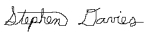
\includegraphics[scale=1]{stephsig.jpg}} \\
\fromname{Stephen Davies \\ Professor, Computer Science}
}
\end{letter}
\end{document}
